\section{Introduction}

Agentic applications call a language model many times per task, so the price of a call is multiplied by the length
of the loop. Belcak et al.~\cite{belcak2025slm} argue that small language models are sufficient for most of these
calls, more suitable and cheaper, and that agentic systems should use them by default and invoke large models
``selectively and sparingly''. The paper is a position paper: its evidence is cited from benchmark results of
individual models, and the routing mechanism its architecture depends on is left open.

We ask the question empirically, in the setting where the position should be easiest to confirm: open models from
0.23B to 27B active parameters on tool-use tasks with a controlled harness. We test three ways to make a small model
pay in an agentic loop. \emph{Escalation} sends a failing episode to a large model. \emph{Harness routing} gives each
model the scaffold that suits it: worked examples, instructions, a watchdog, constrained decoding. \emph{Delegation}
lets a large model plan and a small model execute each step, and, in its cheapest form, a small model plan as well.

Every stage was pre-registered before its first episode, with hypotheses, decision rules and analysis, and every
later change is in a dated log. Every decision rule was also run on copies of the data whose labels were shuffled
among the compared systems, and a superiority verdict counts only when its rule passes at most 5\% of the copies.
This calibration removed two verdicts that the bootstrap intervals alone would have accepted.

Our findings, in order:
\begin{itemize}
  \item Models of about 4B active parameters solve most of what a 27B model solves at a fraction of the cost;
        replaceability falls off below about 1.5B (\S\ref{sec:replace}).
  \item The tool-call parser can erase a model, and harness fixes are model-specific: a finding about instructions
        replicated out of sample, one about worked examples did not (\S\ref{sec:harness}).
  \item A large planner levels small executors, feedback is what makes it work, and the planner is nearly all the
        cost (\S\ref{sec:delegate}).
  \item Prompted small planners break their protocol; a cheap plan lifts weak executors and hurts strong ones; a router
        that plans only after a failure beats always planning, but its gain over a single model is not shown
        (\S\ref{sec:cheap}).
\end{itemize}

\section{Related Work}

\paragraph{Small models in agents.} The position of Belcak et al.~\cite{belcak2025slm} is that SLMs below about 10B
parameters suffice for most agentic calls; its supporting numbers come from model reports, and its LLM-to-SLM
conversion recipe fine-tunes a small model per task cluster. Planner--executor systems built from small models
work when their roles are trained: $\alpha$-UMi~\cite{shen2024alphaumi} fine-tunes a planner, a caller and a summarizer;
Plan-and-Act~\cite{erdogan2025planact} and TinyAgent~\cite{erdogan2024tinyagent} fine-tune the planner;
ToolOrchestra~\cite{toolorchestra2025} trains an 8B orchestrator with reinforcement learning. Plan-first designs such
as ReWOO~\cite{xu2023rewoo} and LLMCompiler~\cite{kim2024llmcompiler} separate planning from tool execution to save
calls. We test the untrained, prompted case, which is what a practitioner gets without a training pipeline.

\paragraph{Routing and cascades.} FrugalGPT~\cite{chen2023frugalgpt} cascades through models of rising cost,
AutoMix~\cite{aggarwal2024automix} escalates when a small model's self-verification is doubtful, and
RouteLLM~\cite{ong2025routellm} learns a router between a strong and a weak model from preference data. These work
on single-turn queries; we route whole agentic episodes, and we route harnesses and plans as well as models.

\section{Setup}\label{sec:setup}

\paragraph{Tracks.} \emph{Code}: MBPP~\cite{austin2021mbpp}, 497 tasks, graded by the reference tests.
\emph{Tools}: BFCL v3 single-turn~\cite{patil2025bfcl}, 800 tasks. \emph{Shell}: 50 generated multi-step tasks
with \texttt{bash} and \texttt{write\_file}, graded by the final answer or the files left behind. \emph{Multi-turn}: BFCL v4 multi-turn base, 200 tasks on stateful simulators (file system,
messaging, trading, travel, vehicle), where a user makes several requests in one conversation and the simulator state
is checked after each; stage 4 adds the miss-parameter and long-context categories, 200 tasks each. Replaying the
ground truth through our harness scores 1.0 on all 600 multi-turn tasks. Tasks are split once by a hash of their id
into screen (15\%), train (25\%) and test (60\%).

\paragraph{Models.} Twelve models in stages 1--2: MNN-Pocket-0.3B, Qwen3-0.6B, Qwen3.5-0.8B and a weight-edited
variant, Qwen3.5-2B, -4B and -9B, Granite-4.0-micro, Qwen3-VL-8B, and three larger ones served through a gateway
(Gemma-4-26B-A4B, Qwen3-VL-30B-A3B and a 27B dense model we call qwen3.8). Phase L adds seven models that were not
used to form the stage-2 findings: LFM2.5 at 230M, 350M, 1.2B, 2.6B and 8B-A1B, and Gemma-4-E2B and -E4B. Local
models run on vLLM~\cite{kwon2023vllm} at temperature 0.6.

\paragraph{Harness.} The agent sees the task and the tools and calls one or more tools per step until it calls
\texttt{finish}, within a step and token budget per track. Harness components combine freely: \texttt{memory} (three
worked examples of a strong model on the nearest train tasks), \texttt{skill} (a per-track how-to, loaded on demand)
or \texttt{skill\_inline} (in the prompt), \texttt{watchdog} (nudges on repeats, broken calls and runaway output) and
\texttt{strict} (calls constrained to the tools' JSON schema).

\paragraph{Cost.} An episode costs $2\,N_\text{active}\,(t_\text{prompt}+t_\text{completion})$ FLOPs, summed over its
calls and, under delegation, over planner and executor. It counts prompt tokens in full, so it ignores prefix
caching, and it counts a model's thinking tokens.

\paragraph{Statistics.} Quality is the macro pass rate over tracks. Differences are paired by task, with a 95\%
bootstrap within track and a sign-flip permutation $p$. Wherever a rule chooses among options (a threshold, a
harness, a router) it chooses on fit data (screen and train, or other cross-validation folds) and is scored on held-out
tasks. The \nHypotheses{} verdicts are in Appendix~\ref{app:verdicts}.

\section{Small Models Replace Large Ones, Up to a Point}\label{sec:replace}

Figure~\ref{fig:replace} shows, for each model, the share of the test tasks solved by qwen3.8 that the model also
solves alone. Qwen3.5-9B solves \replNineMT{} of them on multi-turn, \replNineShell{} on shell and \replNineCode{} on
code, at a \costNine$\times$ lower cost per task; Qwen3.5-4B solves \replFourMT{}, \replFourShell{} and \replFourCode{}
at \costFour$\times$. What matters is active parameters: Qwen3-VL-30B, a mixture of experts with 3B active,
replaces \replVlThirtyMT{}, \replVlThirtyShell{} and \replVlThirtyCode{} at \costVlThirty$\times$. Below about 1.5B
active parameters replaceability collapses on the agentic tracks (LFM2.5-1.2B: \replLfmOneMT{} multi-turn,
\replLfmOneShell{} shell), though not on single-call tool use. Small models do not make up for their size with longer
episodes: the cost ratio per task is close to the ratio of active parameters or above it, because the 27B model
thinks at length.

\begin{figure}
  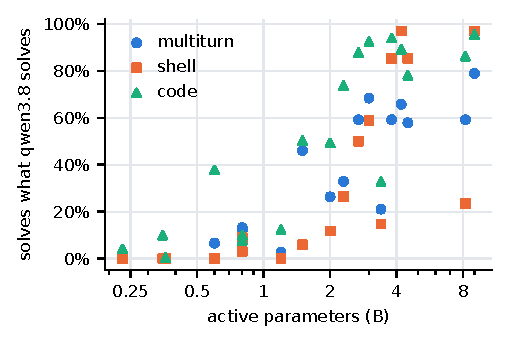
\includegraphics[width=\columnwidth]{figures/replaceability}
  \caption{Share of the test tasks solved by the 27B model that each model also solves alone, by its active
  parameters (log scale).}\label{fig:replace}
\end{figure}

\section{The Harness Is Part of the Model}\label{sec:harness}

\paragraph{The parser.} Runs made under earlier parser versions were set aside and rerun when the parser changed.
On the same \gemmaN{} tasks, Gemma-4-26B solved \gemmaOld{} under a parser that did not read its
\texttt{call:name\{\ldots\}} format and \gemmaNew{} under the final parser (\gemmaDiff\pp{}, \gemmaCI). Once a model's
call shape is read, making the parser more lenient mostly changes the count of ``broken'' steps, not the pass rate:
qwen3.8's broken steps fell from \qwenBrokenOld{} to \qwenBrokenNew{} while its quality moved within the noise
(Appendix~\ref{app:parser}). Any comparison of small models is first a comparison of the parsers that read them.

\paragraph{Harness fixes do not transfer.} Stage 2 found, on the twelve stage-1 models, that worked examples
(\texttt{memory}) help small models and that instructions help only large ones. Phase L tested both on seven new
models. Instructions did not help the new small models (mean lift \instrNew\pp{} against \instrGateway\pp{} for the
three large models; gap \instrGap\pp{}, \instrGapCI), which replicates. Worked examples helped only \memoryHelps{} of
the 7, against the pre-registered 5, which does not. The pre-registered router that assigns each model its harness
by rule was not non-inferior to a search over harnesses, and the instruction file that made some stage-2 models
cheaper made six of the seven new ones dearer.

\paragraph{Retry with another harness.} What does help is to change the harness when a small model fails: in a
cascade that stops a flagged episode after two steps and retries it, retrying Qwen3.5-4B with its own best harness beats
a plain retry by \switchLo{} to \switchHi\pp{} at all six budgets. This rule passed \switchFalse{} of shuffled copies, after
we found and fixed two selection effects in the cascade code that had let it pass 48\% (logged in the
pre-registration; Appendix~\ref{app:calibration}).

\section{Delegation Levels Executors, at a Price}\label{sec:delegate}

In stage 3 qwen3.8 plans with thinking off: it sees the task, the tools and a report of every step, and writes one
step at a time as JSON. A small executor sees only that step, the tools it names and up to two worked calls, and has
three turns.

\begin{figure}
  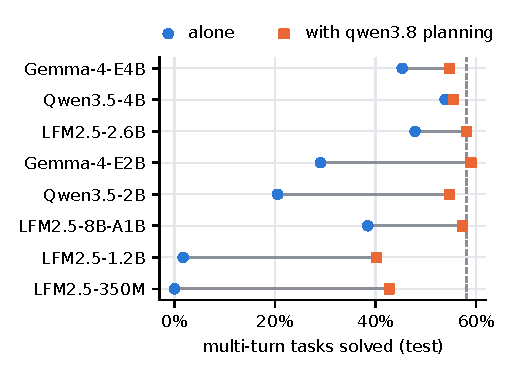
\includegraphics[width=\columnwidth]{figures/levelling}
  \caption{Multi-turn tasks solved (test) by each executor alone and under qwen3.8's plan. The dashed line is
  qwen3.8 executing its own plan.}\label{fig:level}
\end{figure}

A plan levels the executors (Figure~\ref{fig:level}). From 1.5B active parameters up, every executor reaches
\levelLo--\levelHi{} of multi-turn tasks, close to the \pbMT{} of qwen3.8 executing its own plan, whatever it solves alone; the
350M model goes from \tinyAloneMT{} to \tinyPlanMT{}. The plan is the ceiling: a strong executor gains little
(Qwen3.5-4B, \fourAloneMT{} to \fourPlanMT{}). Feedback is what makes it work: when the planner writes the whole plan
at once and does not see the results, quality falls by \feedbackSmall\pp{} for LFM2.5-1.2B and \feedbackFour\pp{}
for Qwen3.5-4B. Worked calls help the weak executor (\examplesSmall\pp{}) but not the strong one (\examplesFour\pp{}).

None of the pre-registered delegation hypotheses held. The best executor of at most 4B active parameters, chosen on
fit, is \bestVsPB\pp{} behind qwen3.8 in the executor seat (\bestVsPBCI): compatible with no loss, but the margin of
5\pp{} is not excluded with 36 shell tasks. And the planner is \plannerShareLo{} or more of the compute of every
delegated episode, so at the cost of a delegated episode a single mid-sized model solves as much or more.

\section{Cheap Planners and a Router}\label{sec:cheap}

Stage 4 asks whether delegation pays with a cheaper planner: \emph{A}, Qwen3.5-9B or -4B planning, used only when
the executor fails alone (a router), against \emph{B}, a tiny stack with LFM2.5-2.6B planning for LFM2.5-350M. It
runs on all 650 tasks, with every router fitted on other folds.

\begin{figure}
  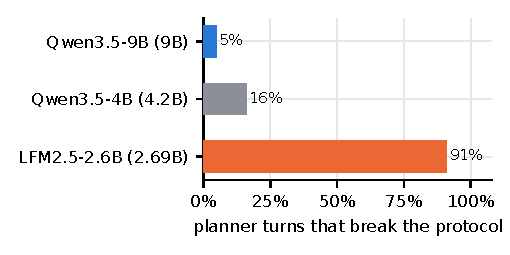
\includegraphics[width=\columnwidth]{figures/protocol}
  \caption{Planner turns that are not a valid step or finish, by the planner's size (stage 4, all executors).}\label{fig:protocol}
\end{figure}

\paragraph{Prompted small planners do not hold the role.} The share of planner turns that are not a valid step
falls with size, \protoLfm{}, \protoFour{} and \protoNine{} for 2.6B, 4B and 9B (Figure~\ref{fig:protocol}). The
2.6B planner calls the tools itself in its native format instead of writing steps, and the tiny stack solves
\tinyStackQ{} of the tasks, \tinyStackVsAlone\pp{} (\tinyStackVsAloneCI) below LFM2.5-2.6B working alone. The same
happens when LFM2.5-2.6B plans for itself, so the failure is the planner's.

\paragraph{A cheap plan helps the weak and hurts the strong.} Planned by Qwen3.5-9B, LFM2.5-350M gains \liftTiny\pp{}
(\liftTinyCI), but LFM2.5-2.6B loses \hurtLfm\pp{} and Qwen3.5-4B loses \hurtFour\pp{} (\hurtFourCI), at \planCostFour$\times$ the cost. The router turns this into a gain over planning always: it keeps the strong model alone where
it succeeds, and R(4B;\,9B) beats always-planned Qwen3.5-4B by \routerVsPlan\pp{} (\routerVsPlanCI) at \routerCost{}
of its cost.

\begin{figure}
  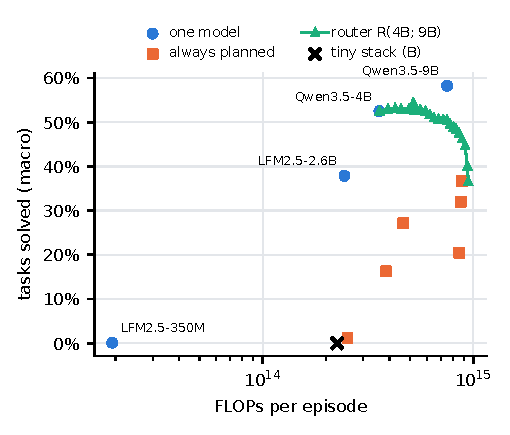
\includegraphics[width=\columnwidth]{figures/frontier}
  \caption{Stage 4: cost per episode against quality for single models, always-planned executors, the router
  R(4B;\,9B) over its thresholds, and the tiny stack.}\label{fig:frontier}
\end{figure}

\paragraph{The router does not beat the best single model.} Against the best single model at the same cost, the best
router gains \routerVsSingle\pp{} (\routerVsSingleCI) at one budget, but the rule that asks for such a gain at any of 16
budgets passed \cpFourFalse{} of shuffled copies, so the gain is not shown; at the highest budget, Qwen3.5-9B alone
is ahead (Figure~\ref{fig:frontier}).

\section{Discussion}

\paragraph{When a small model pays.} A small model pays when it does the whole task alone: a 4B model is a cheap
substitute for a 27B model on most agentic tasks. It does not pay as the executor of a large planner, whose cost
dominates, and a prompted small planner does not work at all. These results support the position that SLMs suffice
for many agentic calls, and they locate its weak point in the part the position leaves to future work: planning and
routing. The systems where small planners work fine-tune them~\cite{shen2024alphaumi,erdogan2025planact,erdogan2024tinyagent,toolorchestra2025},
as does the conversion recipe of~\cite{belcak2025slm}; our results say that this training is not optional.

\paragraph{What routing is for.} A router's value here was defensive: it kept a strong model from a plan that hurt
it. A router that adds quality over the best single model at equal cost was not shown, and the calibration showed
why such claims need care: a rule that may pick its best budget out of many passes too often on noise.

\paragraph{Limitations.} One sample per task at temperature 0.6; the shell track has 36 test tasks, which limits
non-inferiority claims; FLOPs ignore prefix caching, which would lower the planner's cost; the router evaluation
restarts a task from scratch, which simulators allow and side-effecting tasks do not; models were served on shared
GPUs, which affects latency, not outcomes. Several analysis choices were corrected after their freeze; each is
dated in the pre-registration logs, and none changed a verdict except the two removed by calibration.

\section{Conclusion}

Small models are good substitutes for large ones on agentic tasks at a fraction of the cost, but the harness that
reads them matters as much as the model, harness fixes do not transfer between models, and cheap delegation does
not pay without trained planners. \release

\paragraph{Disclosure.} The author used an AI assistant (Claude) to write experiment and analysis code, to run
experiments and to draft this text; every number is generated from the released logs by the released scripts.
